\documentclass{beamer}

\usepackage[utf8]{inputenc}
\usepackage[T1]{fontenc}
\usepackage{amsmath}
\usepackage{bm}

\usepackage{tabularx}
\usepackage{graphicx}
\usepackage{epstopdf}
\usepackage{natbib}
\usepackage{multirow}

\graphicspath{{../../images/}}

\usetheme{Madrid}
\usebeamercolor{sidebartab}
\usefonttheme{professionalfonts}


\title[M.Sc. Thesis 2015]{Spatial Summarization of Image Collections}
\author{Diego A. Ballesteros Villamizar}
\institute[ETHZ]{ETH Zürich}
\date{January 27th, 2016}

\DeclareMathOperator*{\argmin}{argmin}
\DeclareMathOperator*{\argmax}{argmax}

\AtBeginSection[]
{
  \begin{frame}<beamer>
    \frametitle{Outline}
    \tableofcontents[currentsection]
  \end{frame}
}

\begin{document}

\begin{frame}
  \titlepage
\end{frame}

\section{Featurized FLID}

\begin{frame}{Correct normalization}
  \begin{enumerate}
    \item In previous presentation, latitude and longitude were normalized to full range, i.e. $[-90, 90]$ and $[-180, 180]$ respectively.
    \item All features normalized to $[0, 1]$ range \textbf{over the data}.
    \item However, no improvement of score.
    \item Moreover, the phenomena previously seen on the $bm{W}$ weights is still present, i.e. they are the same across dimensions $d$.
  \end{enumerate}
\end{frame}

\begin{frame}{Why uniform weights across dimensions?}
  \begin{enumerate}
    \item \textit{Note 1:} Initialization of the $\bm{B}$ weights is obtained from a uniform distribution over $[0, 0.001]$.
    \item \textit{Note 2:} The gradient update for $\bm{B}$ is given by equations \ref{eq:update} and \ref{eq:update_argmax}:
      \begin{align}
        \left(\nabla_{\bm{B}} \log{\frac{1}{\hat{Z}} \tilde{P}\left(S \mid \bm{a},\bm{B} \right)}\right)_{m, l} &= x_{i^{*},m} - \sum_{i \in S}{x_{i,m}} 
        \label{eq:update} \\
        i^{*} &= \argmax_{i \in S} \bm{x}_{i} \bm{b}_{l}
        \label{eq:update_argmax}
      \end{align}
      Which shows that the only difference in the weights across dimensions is given by the value of $i^{*}$.
    \item Because the initialization is small in comparison with the feature values and the variability is low, the value of $i^{*}$ at every timestep is equal in all dimensions $d$ as it only depends on the feature vector $\bm{x}_{i}$.
  \end{enumerate}
\end{frame}

\begin{frame}{Fixing weight $\bm{B}$ distribution}
  \begin{enumerate}
    \item To avoid initial updates choosing always the same $i^{*}$, the initialization for $\bm{B}$ should be larger. The new range is $[0, 1]$.
    \item The learned weight matrix $\bm{W}$ is not uniform  with the updated initialization condition.

    \begin{figure}[h]
      \centering
      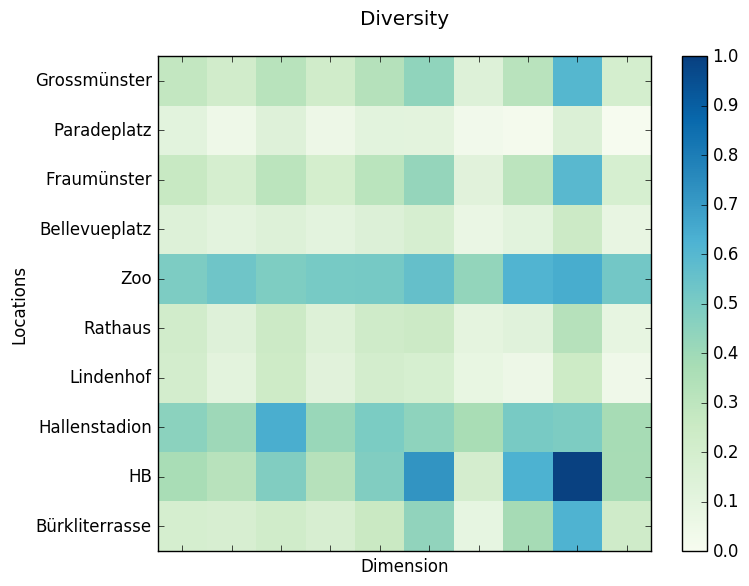
\includegraphics[width=0.5\textwidth]{submodular_weights_f_1_l_dim_10_k_dim_0}
    \end{figure}

  \end{enumerate}
\end{frame}

\begin{frame}{Fixing weight $\bm{B}$ distribution}
  \begin{enumerate}
     \item However, the scoring remains low. Worse than the score with the identity as feature matrix, i.e. the non-featurized model.
     
     \begin{table}
       \centering
       \begin{tabular}{@{}lll@{}}
         \hline
         \textbf{Model} & \textbf{Accuracy} & \textbf{MRR} \\
         \hline
         Modular with features & $17.38 \pm 1.81$ & $39.85 \pm 1.52$ \\
         \textbf{FLID (d = 10)} & $\bm{29.31 \pm 2.74}$ & $\bm{52.19 \pm 1.78}$ \\
         FFLID (d = 1) & $13.60 \pm 1.60$ & $37.54 \pm 1.39$ \\
         FFLID (d = 5) & $13.48 \pm 1.61$ & $37.51 \pm 1.45$ \\
         FFLID (d = 10) & $12.34 \pm 1.51$ & $36.94 \pm 1.47$ \\
         \hline
       \end{tabular}
      \end{table}
  \end{enumerate}
\end{frame}


\section{Extending the Model}

\begin{frame}{Coherence term}
  \begin{align}
    P(S \mid \bm{a}, \bm{B}, \bm{C}) &= \frac{1}{Z} \exp{\left(\sum_{i \in S}{u_{i}} + Div(S,\bm{B}) + Coh(S,\bm{C})\right)} \\
    Div(S,\bm{B}) &= \sum_{l = 1}^{L}{\left( \max_{i \in S}{\bm{x}_{i}\bm{b}_{l}} - \sum_{i \in S}{\bm{x}_{i}\bm{b}_{l}}\right)} \\
    Coh(S,\bm{C}) &= \sum_{k = 1}^{K}{\left(\sum_{i \in S}{\bm{x}_{i}\bm{c}_{k}} - \max_{i \in S}{\bm{x}_{i}\bm{c}_{k}}\right)} \\
    \bm{u} &= \bm{X}\bm{a} \quad \bm{X} \in \mathbb{R}^{|V| \times M} \quad \bm{u} \in \mathbb{R}^{|V|} \quad \bm{a} \in \mathbb{R}^{M}\\
    \bm{W}_{\bm{B}} &= \bm{X}\bm{B} \quad \bm{B} \in \mathbb{R}^{|M| \times L} \\
    \bm{W}_{\bm{C}} &= \bm{X}\bm{C} \quad \bm{C} \in \mathbb{R}^{|M| \times K} \\
  \end{align}
\end{frame}

\begin{frame}{Intuition}
  \begin{enumerate}
    \item Supermodular term encourages adding similar items, i.e. values with high $w_{c_{i,k}}$ close to the $\max_{i \in S}$.
    \item This is a more natural notion in the setting of touristic places, e.g. someone who visits Fraumünster will likely visit Grossmünster as well.
    \item The learning is analog to the diversity-only case, however more parameters are present so more noise samples should be used. The gradient update is the negative of the equation for the diversity case.
  \end{enumerate}
\end{frame}

\begin{frame}{Zürich Path Data}
  \begin{columns}
    \begin{column}{0.5\columnwidth}
      \begin{table}
        \centering
        \caption{Frequency of Item Sets}
        \begin{tabular}{ll}
          \hline
          Set & Frequency \\
          \hline
          $[0, 2]$ & 101 \\
          $[9, 3]$ & 66 \\
          $[0, 5]$ & 63 \\
          $[2, 5]$ & 62 \\
          $[5, 6]$ & 52 \\
          $[9, 1]$ & 50 \\
          $[2, 6]$ & 49 \\
          $[9, 2]$ & 44 \\
          $[0, 2, 5]$ & 43 \\
          $[0, 3]$ & 41 \\
          \hline
        \end{tabular}
      \end{table}
    \end{column}
    
    \begin{column}{0.5\columnwidth}
      \begin{table}
        \centering
        \caption{Locations}
        \begin{tabular}{ll}
          \hline
          Index & Location \\
          \hline
          0 & Grossmünster \\
          1 & Paradeplatz \\
          2 & Fraumünster \\
          3 & Bellevue \\
          4 & Zoo \\
          5 & Rathaus \\
          6 & Lindenhof \\
          7 & Hallenstadion \\
          8 & HB \\
          9 & Bürkliplatz \\
          \hline
        \end{tabular}
      \end{table}
    \end{column}
  \end{columns}
\end{frame}

\begin{frame}{Model without Features}
  \begin{equation*}
    \bm{X} = \mathbb{I}
  \end{equation*}
  
  \begin{table}
    \begin{tabular}{l|lllll}
      \hline
      & \multicolumn{5}{c}{K} \\
      \hline
      \multirow{5}{*}{L} & & 0 & 2 & 5 & 10 \\
      & 0 & $18.15 \pm 3.08$ & $24.85 \pm 7.37$ & $31.06 \pm 6.89$ & $30.72 \pm 3.22$ \\
      & 2 & $22.39 \pm 2.66$ & $\bm{34.07 \pm 2.63}$ &&\\
      & 5 & $24.04 \pm 3.22$ && $34.35 \pm 2.15$ &\\
      & 10 & $29.31 \pm 2.74$ &&& $35.48 \pm 2.16$ \\
    \end{tabular}
  \end{table}
\end{frame}

\begin{frame}{Model without Features}
  \begin{figure}
    \centering
    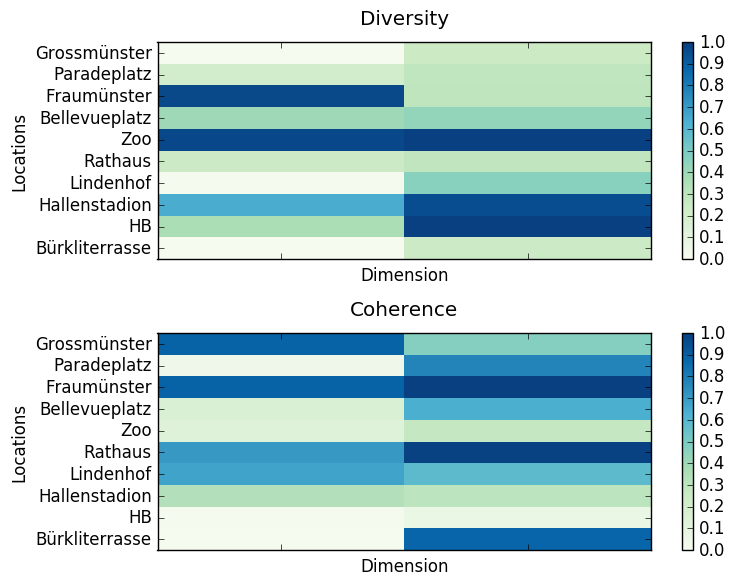
\includegraphics[height=0.8\textheight]{submodular_weights_f_0_l_dim_2_k_dim_2}
  \end{figure}
\end{frame}

\begin{frame}{Model with Features}
  \begin{equation*}
  \bm{X} \in \mathbb{R}^{10 \times 4}
  \end{equation*}
  
  \begin{table}
    \begin{tabular}{l|lllll}
      \hline
      & \multicolumn{5}{c}{K} \\
      \hline
      \multirow{5}{*}{L} & & 0 & 2 & 5 & 10 \\
      & 0 & $17.38 \pm 1.81$ & $16.69 \pm 1.67$ & $16.77 \pm 2.13$ & $17.90 \pm 1.65$ \\
      & 2 & $13.39 \pm 1.58$ & $13.63 \pm 1.64$ &&\\
      & 5 & $13.48 \pm 1.61$ && $13.21 \pm 1.44$ &\\
      & 10 & $12.34 \pm 1.51$ &&& $12.96 \pm 1.14$ \\
    \end{tabular}
  \end{table}
\end{frame}

\begin{frame}{Model with Features}
  \begin{figure}
    \centering
    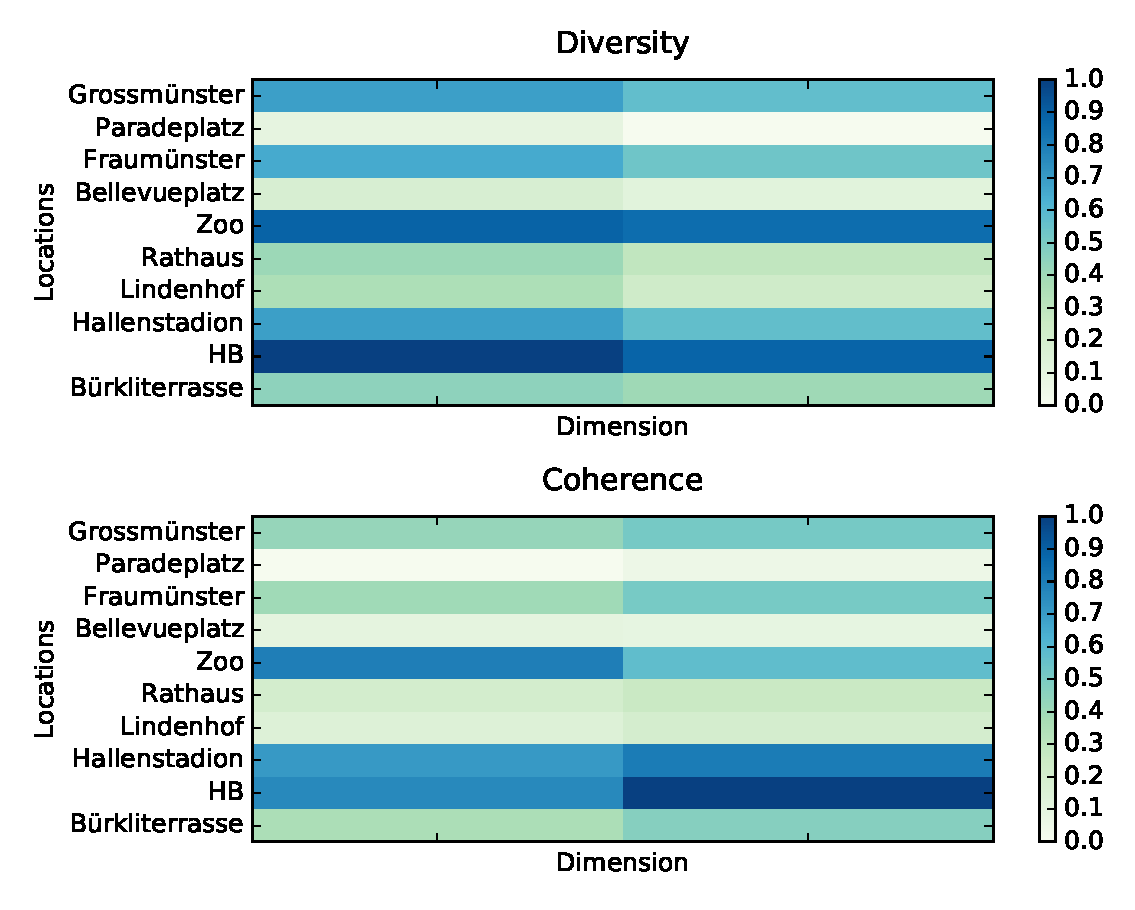
\includegraphics[height=0.8\textheight]{submodular_weights_f_1_l_dim_2_k_dim_2}
  \end{figure}
\end{frame}

\begin{frame}{Experiment Performance}
  \begin{enumerate}
    \item As the number of parameters increase, what is the cost on running time performance?
    \item As in \cite{tschiatschek16learning}, let's define $\kappa = \max_{S \in \mathcal{D} \cup \mathcal{N}}|S|$.
    \item The gradient update operations per iteration are:
    \begin{enumerate}
      \item Updating the utility vector $a$: $O(\kappa M)$.
      \item Updating the weights $B$: $O(\kappa M L)$.
      \item Updating the weights $C$: $O(\kappa M K)$.
    \end{enumerate}
    \item Then the overall performance is: $O(|\mathcal{D} \cup \mathcal{N}| \kappa M (L + K))$.
    \item This is similar to the performance reported on \cite{tschiatschek16learning}: $O(|\mathcal{D} \cup \mathcal{N}| \kappa D)$, as long as $L + K \approx D$ and $M \ll \kappa$.
  \end{enumerate}
\end{frame}

\section{Gaussian Mixture Model}

\begin{frame}{GMM Details}
  \begin{enumerate}
    \item 168607 photos in the Zürich dataset.
    \item EM algorith to learn Gaussian models.
    \item Initial exploration with $k = 10$ clusters. Same cluster number as the previous models.
  \end{enumerate}
  \begin{figure}
    \centering
    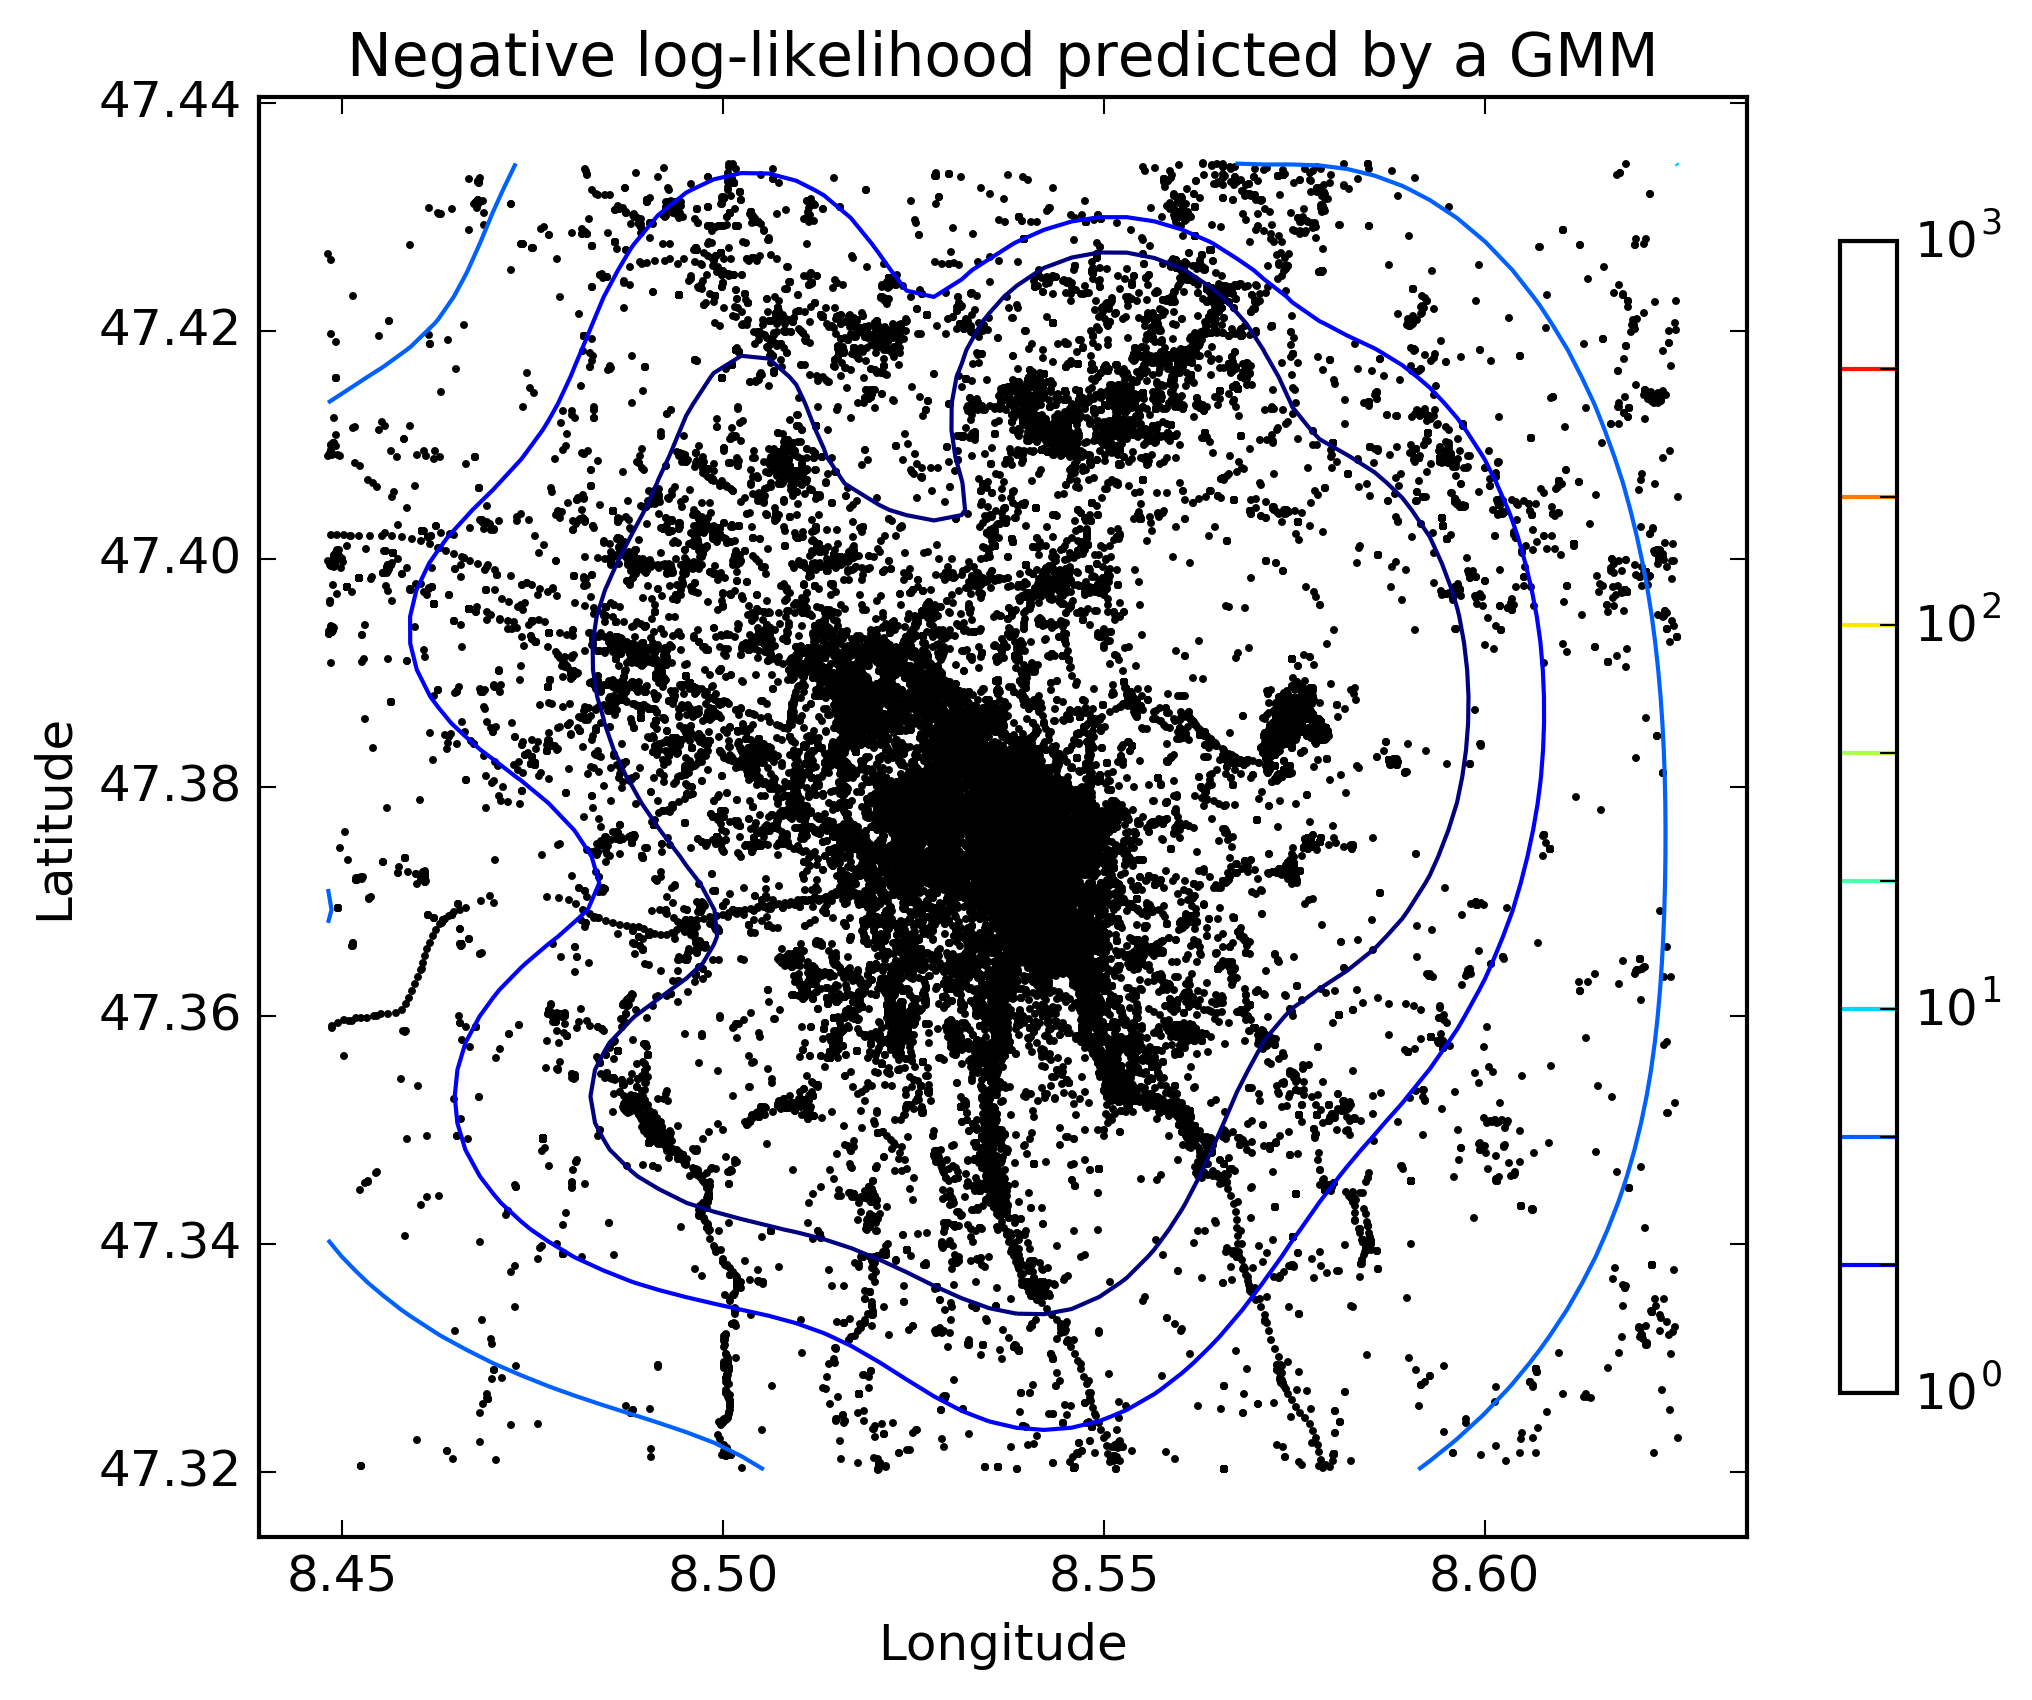
\includegraphics[width=0.5\columnwidth]{gmm_nlog_likelihood}
  \end{figure}
\end{frame}

\begin{frame}{Choosing $k$ using BIC}
  \begin{table}
    \begin{tabular}{ll}
      \hline
      $k$ & BIC score \\
      \hline
      $5$ & $-502347$ \\
      $10$ & $-553062$ \\
      $15$ & $-577692$ \\
      $20$ & $-578098$ \\
      $25$ & $-580983$ \\
      $\bm{30}$ & $\bm{-581246}$ \\
      $40$ & $-581005$ \\
      $50$ & $-580006$ \\
      \hline
    \end{tabular}
  \end{table}
\end{frame}

\begin{frame}{GMM with $k = 30$}
  \begin{columns}
    \begin{column}{0.5\columnwidth}
      \begin{figure}
        \centering
        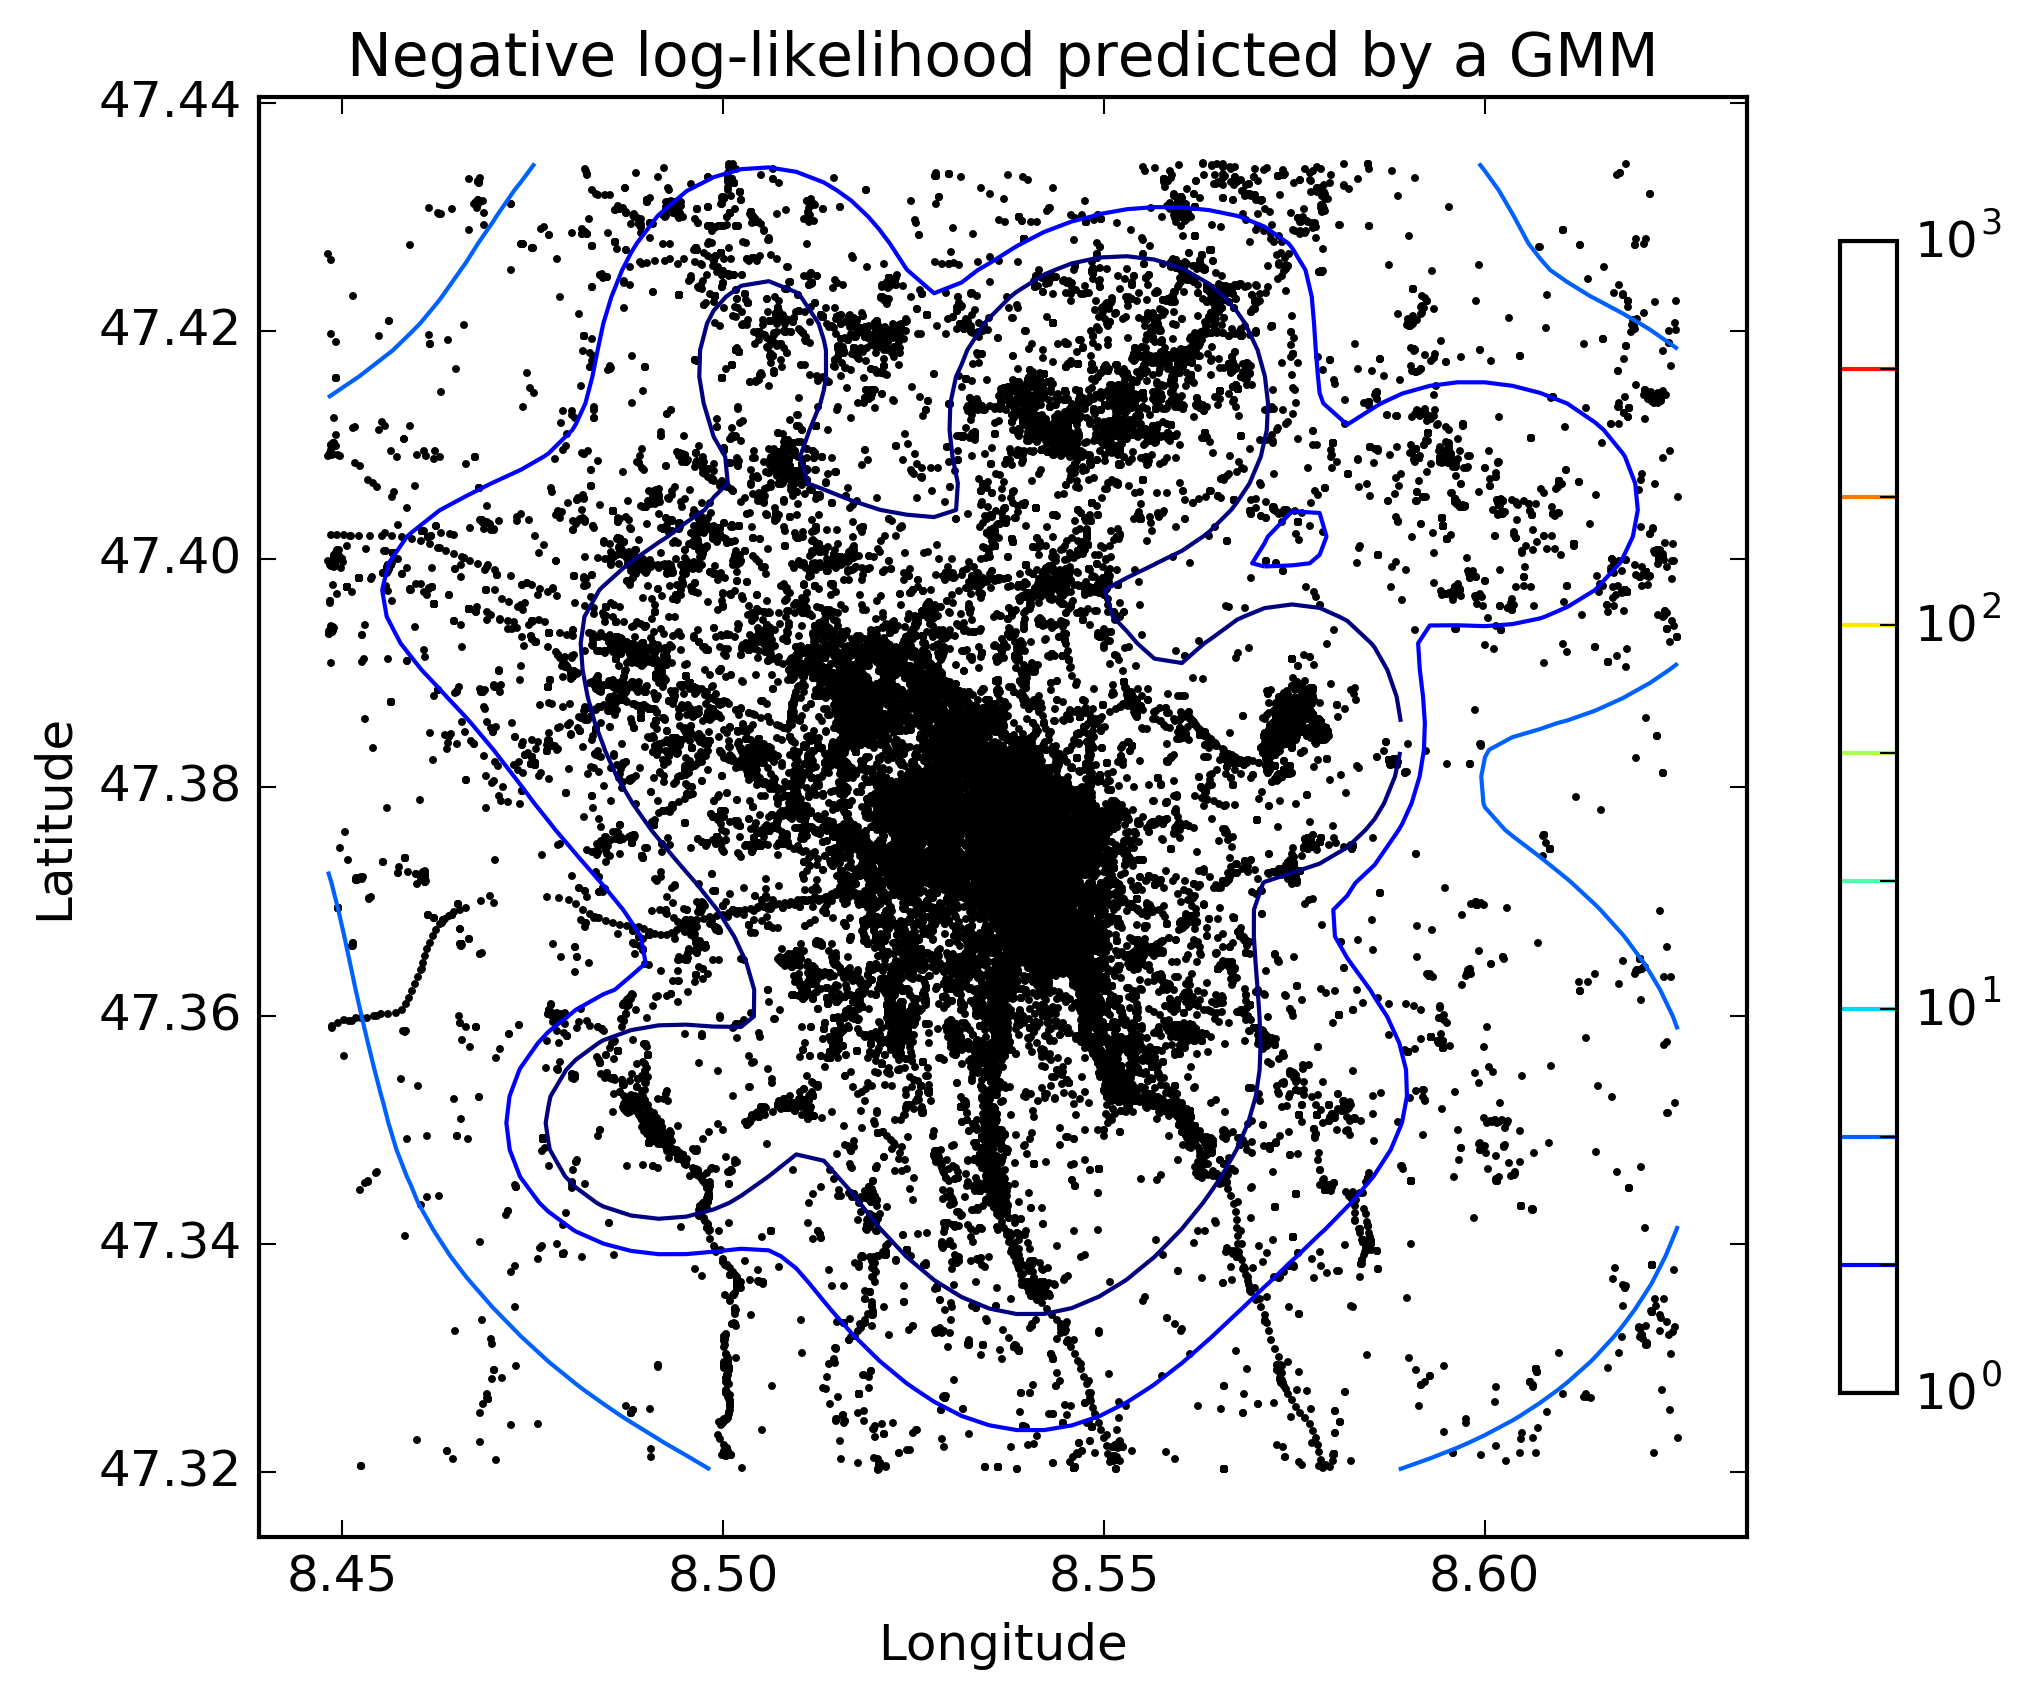
\includegraphics[width=\columnwidth]{gmm_nlog_likelihood_30}
      \end{figure}
    \end{column}
    \begin{column}{0.5\columnwidth}
      \begin{figure}
        \centering
        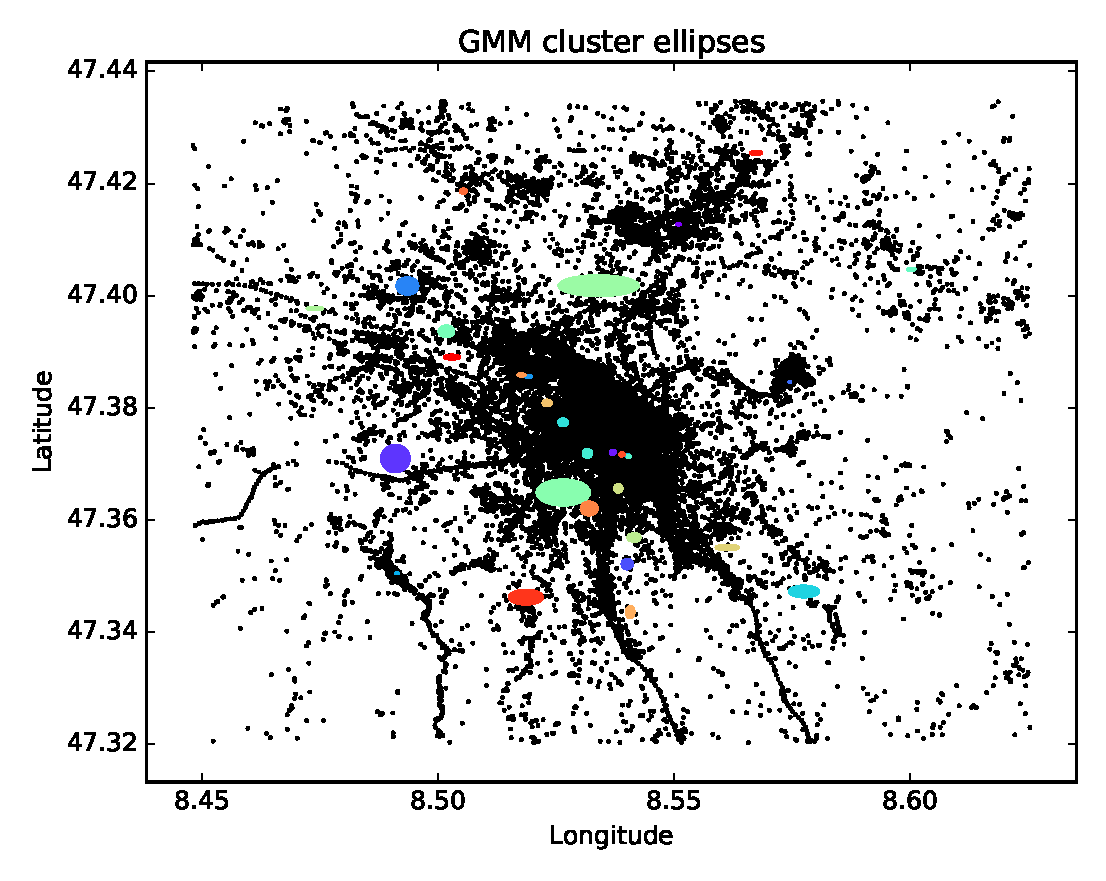
\includegraphics[width=\columnwidth]{gmm_clusters_30}
      \end{figure}
    \end{column}
  \end{columns}
\end{frame}

\begin{frame}{References}
  \bibliographystyle{acm}
  \bibliography{../references.bib}
\end{frame}

\end{document}
